\section{文章增删改}

\subsection{文章详情}

点击主界面的文章链接,即可访问文章详情页.
\begin{figure}[thbp!]
	\centering
	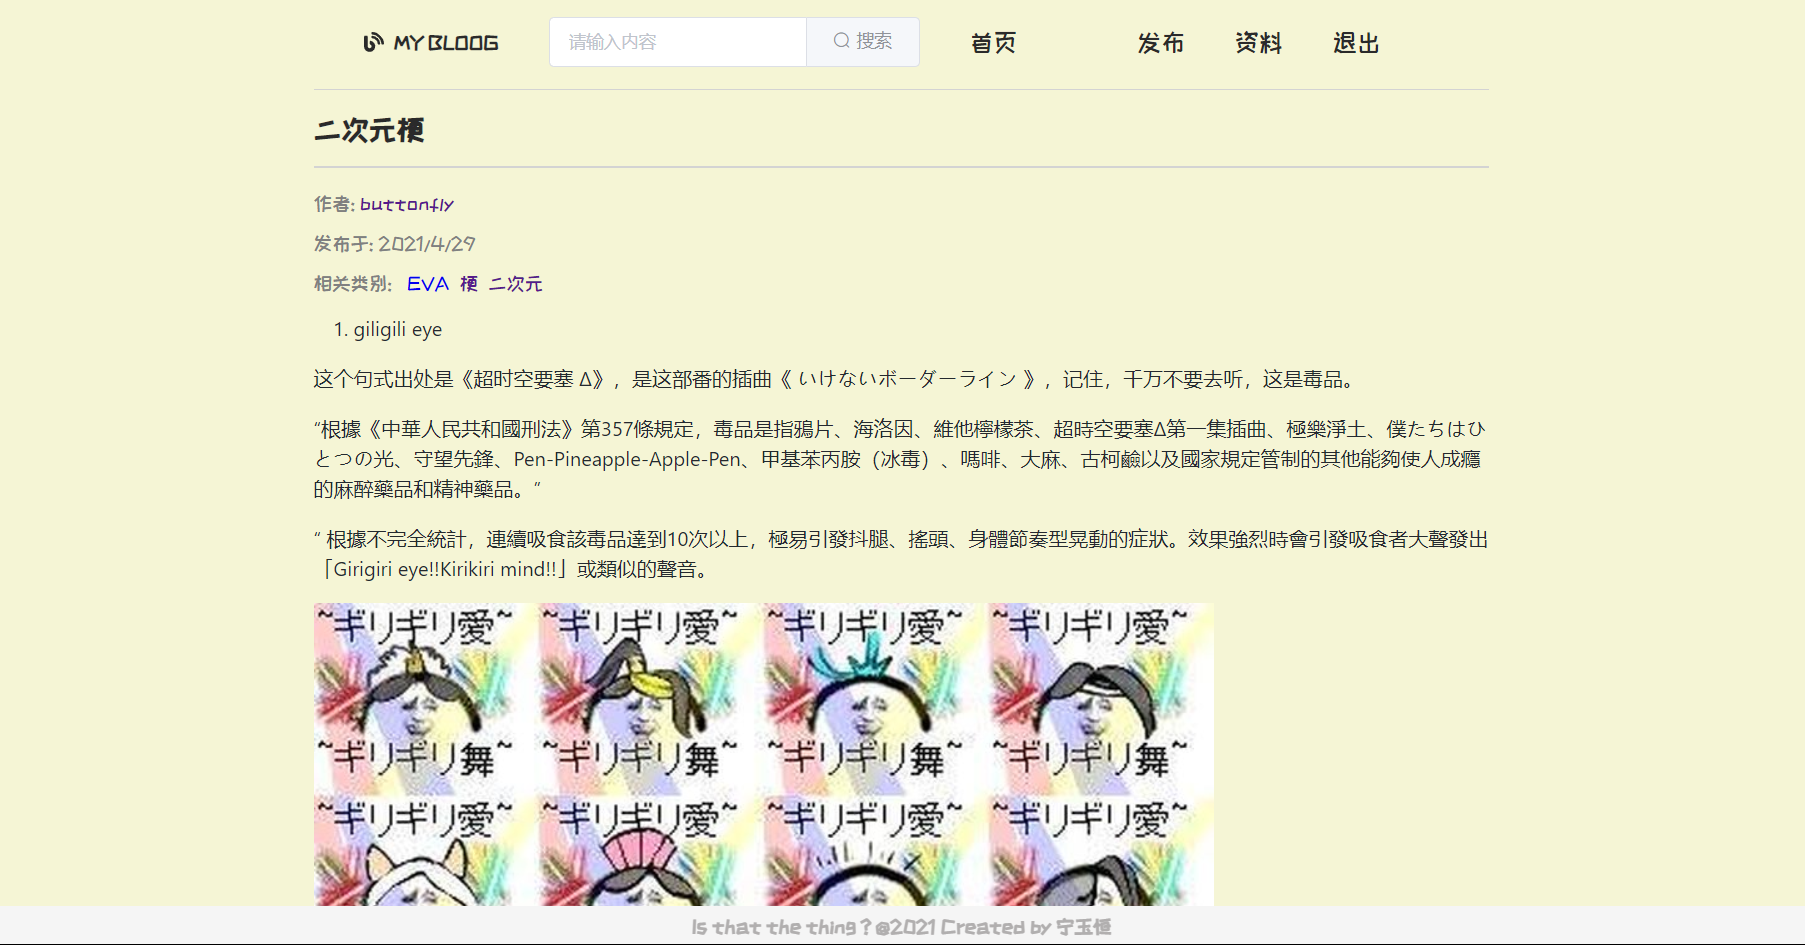
\includegraphics[scale=0.35]{figure/article1}
	\caption{详情页完美支持markdown语法显示}
\end{figure}

\begin{figure}[thbp!]
	\centering
	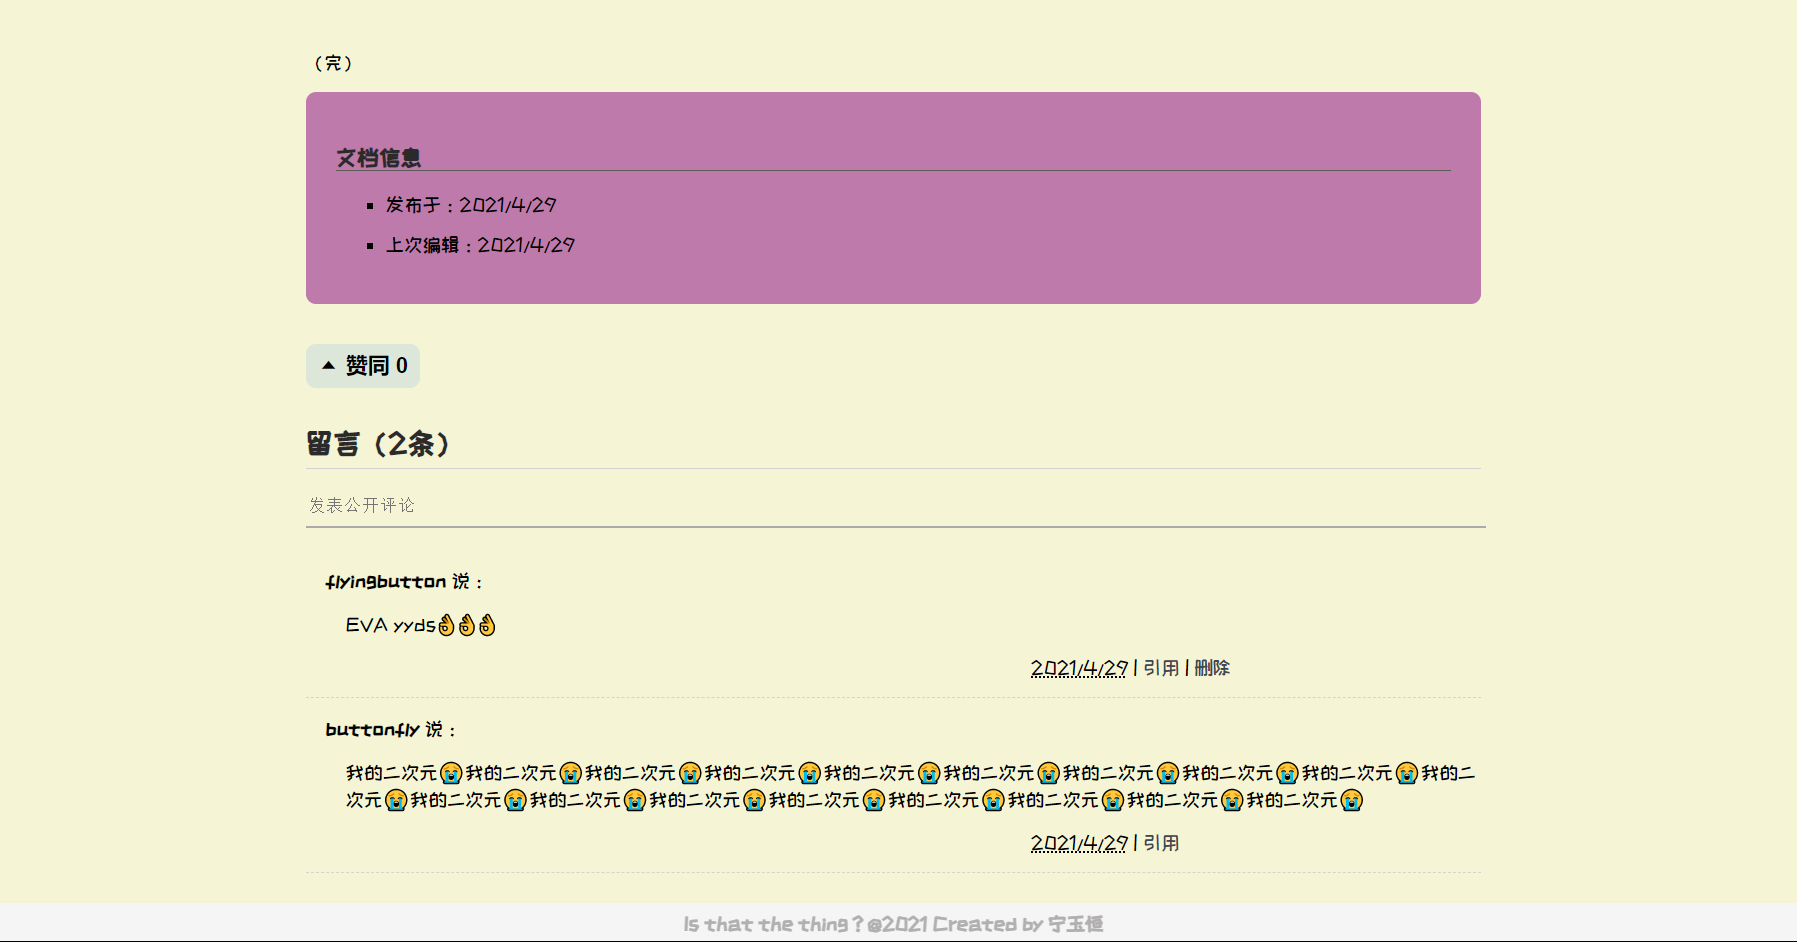
\includegraphics[scale=0.35]{figure/article2}
	\caption{文章支持点赞,留言支持嵌套}
\end{figure}

\subsection{文章发布或删改}

点击界面上方导航栏的发布按钮,即可进入到新文章的编辑.
\begin{figure}[thbp!]
	\centering
	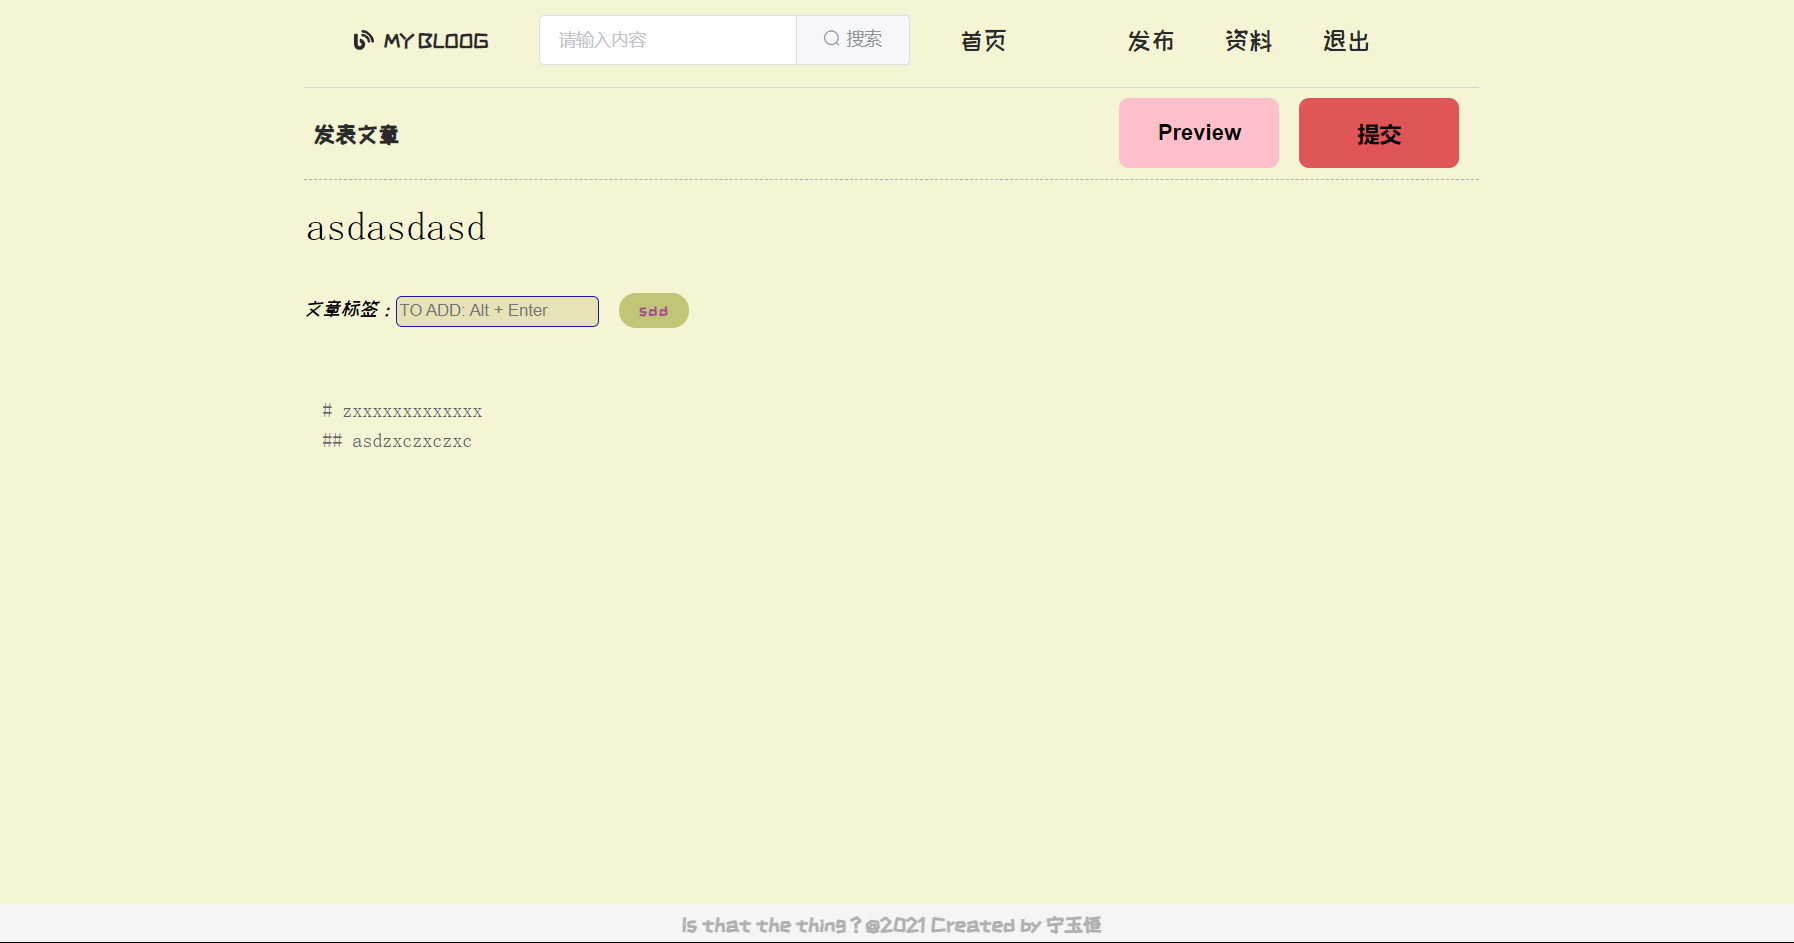
\includegraphics[scale=0.35]{figure/new}
	\caption{文章编辑支持markdown语法,且支持预览,可自定义添加标签}
\end{figure}

修改页面与之类似.
\begin{figure}[thbp!]
	\centering
	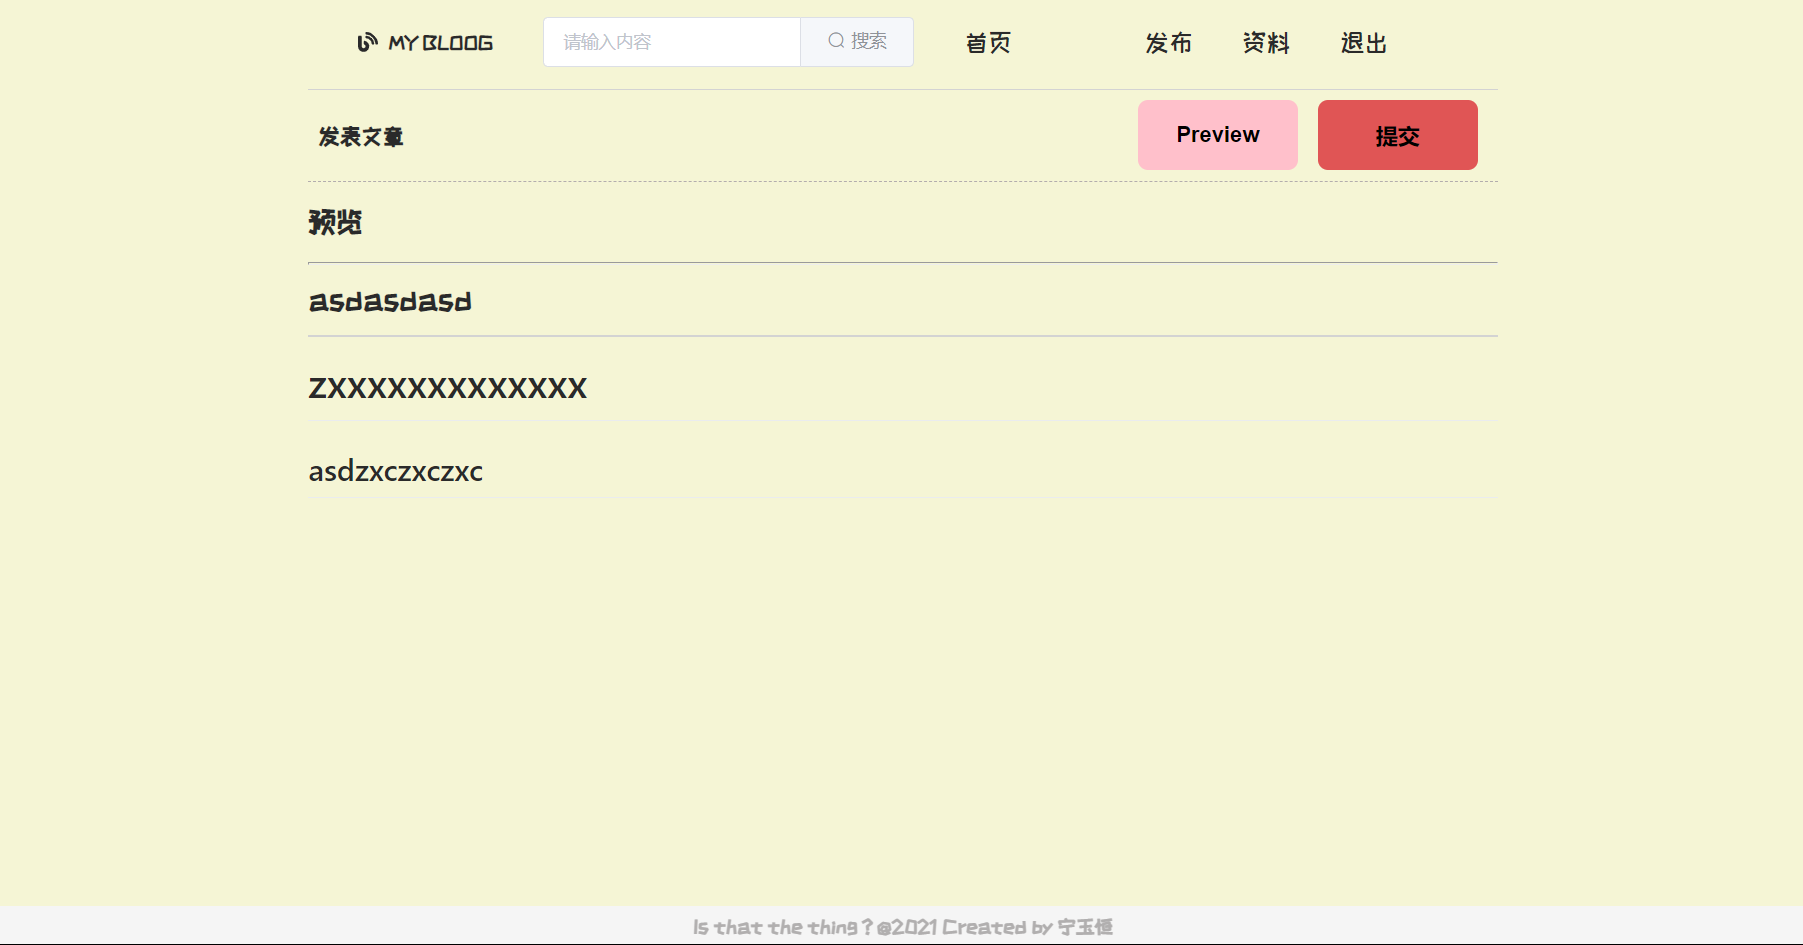
\includegraphics[scale=0.35]{figure/modify}
	\caption{文章内容修改}
\end{figure}

